\documentclass{article}
\usepackage{graphics,indentfirst,amsmath,amsthm,amssymb,latexsym,enumerate}
\usepackage{graphicx}
\usepackage{zed-csp}
%%%%%%%%%%%%%%%%%%%%%%%%%%%%%%%%%%%%%%%%%%%%%%%%%%%%%%%%%%%%%%%%
%  6.826 (POCS Seminar) macro file for handouts and problem sets.
%
% You should save this file as handout.tex
%
% Your main LaTeX file should look like this:
%
%        \documentstyle[12pt]{article}
%
%        %%%%%%%%%%%%%%%%%%%%%%%%%%%%%%%%%%%%%%%%%%%%%%%%%%%%%%%%%%%%%%%%
%  6.826 (POCS Seminar) macro file for handouts and problem sets.
%
% You should save this file as handout.tex
%
% Your main LaTeX file should look like this:
%
%        \documentstyle[12pt]{article}
%
%        %%%%%%%%%%%%%%%%%%%%%%%%%%%%%%%%%%%%%%%%%%%%%%%%%%%%%%%%%%%%%%%%
%  6.826 (POCS Seminar) macro file for handouts and problem sets.
%
% You should save this file as handout.tex
%
% Your main LaTeX file should look like this:
%
%        \documentstyle[12pt]{article}
%
%        \input{handout}
%%%%%%%%%%%%%%%%%%%%%%%%%%%%%%%%%%%%%%%%%%%%%%%%%%%%%%%%%%%%%%%%

\oddsidemargin 0in
\evensidemargin 0in
\marginparwidth 40pt
\marginparsep 10pt
\topmargin 0pt
\headsep 0in
\headheight 0in
\textheight 8.5in
\textwidth 6in
\brokenpenalty=10000

% \handout{number}{date}{title}

\newcommand{\handout}[3]{


\begin{center}
\rule{\textwidth}{.0075in} \\
\rule[3mm]{\textwidth}{.0075in}\\

CMU 17-651\hfill Models of Software Systems\hfill Fall 2018\\[3ex]

{\Large\bf #3}\\[3ex]

Dario A Lencina-Talarico \hfill {\bf Handout #1} \hfill #2

\rule{\textwidth}{.0075in} \\
\rule[3mm]{\textwidth}{.0075in} \\
\end{center}

}

% \homework{number}{date}{title}{due-date}
\newcommand{\homework}[4]{

\begin{center}
\rule{\textwidth}{.0075in} \\
\rule[3mm]{\textwidth}{.0075in}\\

CMU 17-651\hfill Models of Software Systems\hfill Fall 2018\\[3ex]

{\Large\bf #3} \\[3ex]

Dario A Lencina Talarico \hfill  #1  \hfill Due: #2\\

\rule{\textwidth}{.0075in} \\
\rule[3mm]{\textwidth}{.0075in} \\
\end{center}

%\noindent
%{\bf Due date: #4}

}

% \solutionset{number}{date}{title}{due-date}
\newcommand{\solutionset}[4]{

\begin{center}
\rule{\textwidth}{.0075in} \\
\rule[3mm]{\textwidth}{.0075in}\\

CMU 17-651\hfill Models of Software Systems\hfill Fall 2016\\[3ex]

{\Large\bf #3} \\[3ex]

Garlan  \hfill  Solutions for Homework #1  \hfill  #2\\

\rule{\textwidth}{.0075in} \\
\rule[3mm]{\textwidth}{.0075in} \\
\end{center}

%\noindent
%{\bf Due date: #4}

}

% \problem{problem-number}
\newcommand{\problem}[1]{
\vspace{2ex}
\noindent
{\bf Problem #1.}

}

% \solution{solution-number}{points}
\newcommand{\solution}[2]{
\vspace{3ex}
\noindent
{\bf Problem #1}  (#2 points)

}

\newcommand{\cscomment}{
\vspace{1ex}
\noindent Comments: }

% \parts{part-alphabet}{points}
\newcommand{\parts}[2]{
\vspace{2ex}
\noindent
{\bf (#1)}  (#2 points)

}

% \problems{problems-number}{points}
\newcommand{\problems}[2]{
\vspace{3ex}
\noindent
{\bf Problem #1}  (#2 points)

}

\newenvironment{symbolfootnotes}{\def\thefootnote{\fnsymbol{footnote}}}{}

%%%%%%%%%%%%%%%%%%%%%%%%%%%%%%%%%%%%%%%%%%%%%%%%%%%%%%%%%%%%%%%%

\oddsidemargin 0in
\evensidemargin 0in
\marginparwidth 40pt
\marginparsep 10pt
\topmargin 0pt
\headsep 0in
\headheight 0in
\textheight 8.5in
\textwidth 6in
\brokenpenalty=10000

% \handout{number}{date}{title}

\newcommand{\handout}[3]{


\begin{center}
\rule{\textwidth}{.0075in} \\
\rule[3mm]{\textwidth}{.0075in}\\

CMU 17-651\hfill Models of Software Systems\hfill Fall 2018\\[3ex]

{\Large\bf #3}\\[3ex]

Dario A Lencina-Talarico \hfill {\bf Handout #1} \hfill #2

\rule{\textwidth}{.0075in} \\
\rule[3mm]{\textwidth}{.0075in} \\
\end{center}

}

% \homework{number}{date}{title}{due-date}
\newcommand{\homework}[4]{

\begin{center}
\rule{\textwidth}{.0075in} \\
\rule[3mm]{\textwidth}{.0075in}\\

CMU 17-651\hfill Models of Software Systems\hfill Fall 2018\\[3ex]

{\Large\bf #3} \\[3ex]

Dario A Lencina Talarico \hfill  #1  \hfill Due: #2\\

\rule{\textwidth}{.0075in} \\
\rule[3mm]{\textwidth}{.0075in} \\
\end{center}

%\noindent
%{\bf Due date: #4}

}

% \solutionset{number}{date}{title}{due-date}
\newcommand{\solutionset}[4]{

\begin{center}
\rule{\textwidth}{.0075in} \\
\rule[3mm]{\textwidth}{.0075in}\\

CMU 17-651\hfill Models of Software Systems\hfill Fall 2016\\[3ex]

{\Large\bf #3} \\[3ex]

Garlan  \hfill  Solutions for Homework #1  \hfill  #2\\

\rule{\textwidth}{.0075in} \\
\rule[3mm]{\textwidth}{.0075in} \\
\end{center}

%\noindent
%{\bf Due date: #4}

}

% \problem{problem-number}
\newcommand{\problem}[1]{
\vspace{2ex}
\noindent
{\bf Problem #1.}

}

% \solution{solution-number}{points}
\newcommand{\solution}[2]{
\vspace{3ex}
\noindent
{\bf Problem #1}  (#2 points)

}

\newcommand{\cscomment}{
\vspace{1ex}
\noindent Comments: }

% \parts{part-alphabet}{points}
\newcommand{\parts}[2]{
\vspace{2ex}
\noindent
{\bf (#1)}  (#2 points)

}

% \problems{problems-number}{points}
\newcommand{\problems}[2]{
\vspace{3ex}
\noindent
{\bf Problem #1}  (#2 points)

}

\newenvironment{symbolfootnotes}{\def\thefootnote{\fnsymbol{footnote}}}{}

%%%%%%%%%%%%%%%%%%%%%%%%%%%%%%%%%%%%%%%%%%%%%%%%%%%%%%%%%%%%%%%%

\oddsidemargin 0in
\evensidemargin 0in
\marginparwidth 40pt
\marginparsep 10pt
\topmargin 0pt
\headsep 0in
\headheight 0in
\textheight 8.5in
\textwidth 6in
\brokenpenalty=10000

% \handout{number}{date}{title}

\newcommand{\handout}[3]{


\begin{center}
\rule{\textwidth}{.0075in} \\
\rule[3mm]{\textwidth}{.0075in}\\

CMU 17-651\hfill Models of Software Systems\hfill Fall 2018\\[3ex]

{\Large\bf #3}\\[3ex]

Dario A Lencina-Talarico \hfill {\bf Handout #1} \hfill #2

\rule{\textwidth}{.0075in} \\
\rule[3mm]{\textwidth}{.0075in} \\
\end{center}

}

% \homework{number}{date}{title}{due-date}
\newcommand{\homework}[4]{

\begin{center}
\rule{\textwidth}{.0075in} \\
\rule[3mm]{\textwidth}{.0075in}\\

CMU 17-651\hfill Models of Software Systems\hfill Fall 2018\\[3ex]

{\Large\bf #3} \\[3ex]

Dario A Lencina Talarico \hfill  #1  \hfill Due: #2\\

\rule{\textwidth}{.0075in} \\
\rule[3mm]{\textwidth}{.0075in} \\
\end{center}

%\noindent
%{\bf Due date: #4}

}

% \solutionset{number}{date}{title}{due-date}
\newcommand{\solutionset}[4]{

\begin{center}
\rule{\textwidth}{.0075in} \\
\rule[3mm]{\textwidth}{.0075in}\\

CMU 17-651\hfill Models of Software Systems\hfill Fall 2016\\[3ex]

{\Large\bf #3} \\[3ex]

Garlan  \hfill  Solutions for Homework #1  \hfill  #2\\

\rule{\textwidth}{.0075in} \\
\rule[3mm]{\textwidth}{.0075in} \\
\end{center}

%\noindent
%{\bf Due date: #4}

}

% \problem{problem-number}
\newcommand{\problem}[1]{
\vspace{2ex}
\noindent
{\bf Problem #1.}

}

% \solution{solution-number}{points}
\newcommand{\solution}[2]{
\vspace{3ex}
\noindent
{\bf Problem #1}  (#2 points)

}

\newcommand{\cscomment}{
\vspace{1ex}
\noindent Comments: }

% \parts{part-alphabet}{points}
\newcommand{\parts}[2]{
\vspace{2ex}
\noindent
{\bf (#1)}  (#2 points)

}

% \problems{problems-number}{points}
\newcommand{\problems}[2]{
\vspace{3ex}
\noindent
{\bf Problem #1}  (#2 points)

}

\newenvironment{symbolfootnotes}{\def\thefootnote{\fnsymbol{footnote}}}{}


\begin{document}

\homework{}{8 October 2018}{Homework \#6: State Machines II and FSP}{}

\begin{enumerate}[1.]


\item Consider the answering machine described in HW 5. Write an FSP
specification of {\bf AnsMachine}. (For your answer, include the text of the specification and turn in a diagram drawn by LTSA as an
attachment.)

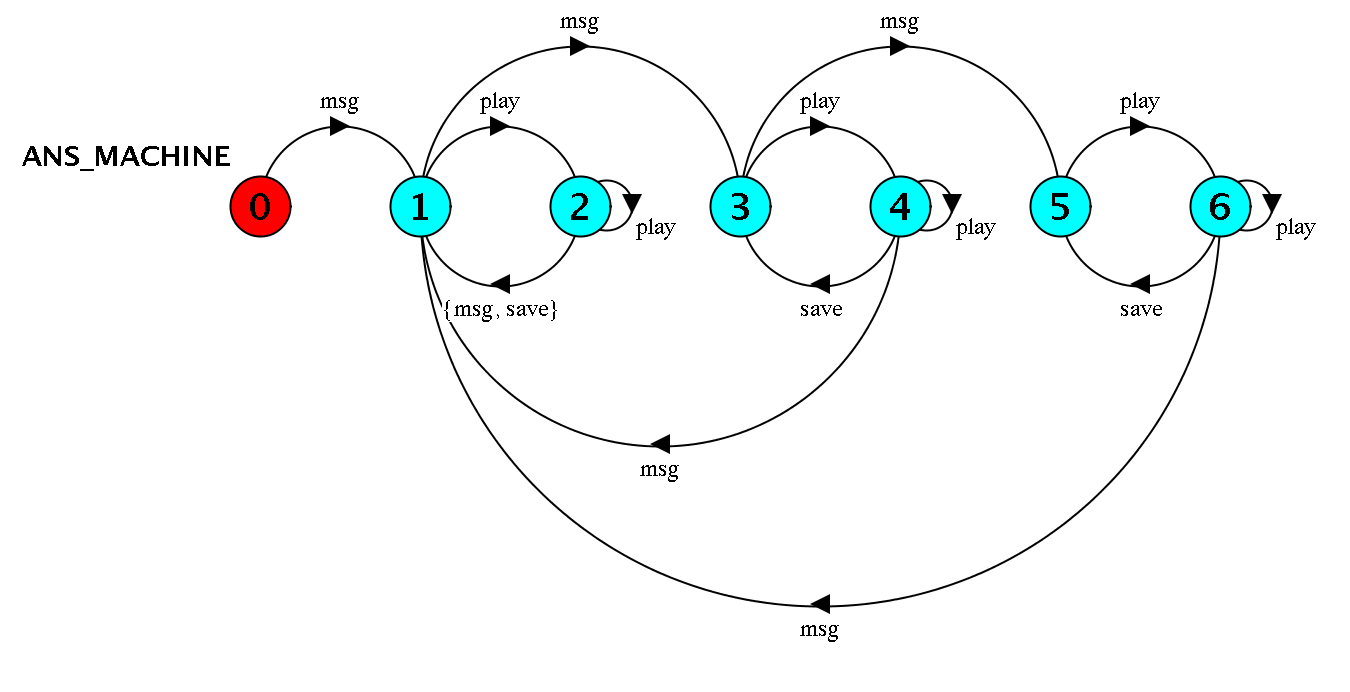
\includegraphics[width=4in]{ans_machine.png}

\begin{verbatim}
ANS_MACHINE = NONE,

NONE = (msg -> ONE),

ONE = (msg -> TWO
      |play -> TEMP1
      ),

TWO = (msg -> THREE
      |play -> TEMP2
      ),

THREE = (play -> TEMP3),

TEMP1 = (play -> TEMP1
        |save -> ONE
        |msg  -> ONE
        ),

TEMP2 = (play -> TEMP2
        |save -> TWO
        |msg  -> ONE
        ),

TEMP3 = (play -> TEMP3
        |save -> THREE
        |msg  -> ONE
        ).
\end{verbatim}


%
%\item Consider the Diverging Counter example of Chapter 10 of GWC09. Prove that $x+y=0$ is an invariant of the $DivergingCounter$ state machine.
%
%(\textsc{Note:} In your proof use style C (in Section 10.1.1) of reasoning about invariants and a similar degree of formalism as in the lecture on this topic.)
%

 \item Consider the FSP specification of a simplified version of the Infusion Pump attached at the end of this assignment.
 Answer the following questions:
    \begin{enumerate}[a.]
    \item Give an example of an action-based trace that causes the infusion pump to terminate without an alarm being raised.
    \item Give an example of an action-based trace that causes the infusion pump to terminate with an alarm being raised.
    \item Is there a limit to how much medication can be administered to a patient? Explain why or why not.
    \item What happens if the nurse forgets to put any medicine in the bag (i.e., uses a refill amount of 0)?
    \item Is it possible for an alarm to sound even if the patient has received the correct and full amount of medicine?
    \end{enumerate}

 \item Modify the FSP specification above to add two of the following capabilities, making sure
 to explain in your comments which capabilities you are adding.
 \begin{enumerate}[a.]
    \item self-check at start-up
    \item confirmation of settings
    \item a start and end of treatment time
    \item other error condition detection
    \item ability to set the amount of medicine to be dispensed at each dispensing step
    \item power outage and automatic switch to backup power supply
    \end{enumerate}
 Submit an electronic copy of the modified FSP specification.
\end{enumerate}

\clearpage

\begin{verbatim}
//---------------------------------------------------
//  Simple Infusion Pump
//---------------------------------------------------

//
// Set of actions that can be selected interactively to
// the animation of this model with the LTSA tool.
//
menu AnimationControlMenu = {
    plug_in, set_value[0..3], reset, fill_fluids
}

//---------------------------------------------------

//======================
// Constants and Ranges
//======================

const Max = 3 range Amt = 0 .. Max

const FillAmt = 2    // Amount in bag initially and after refilling

//=====================
// Process Definitions
//=====================

//
// Pump starts in power off state
//
PUMP = POWER_OFF,

//
// User must plug pump in before anything else can happen
//
POWER_OFF = (
    plug_in -> SETUP
),

//
// Before pump operation starts, user must enter amount of medicine to deliver
// to patient
//
SETUP = (
    set_value[deliver:Amt] -> PUMP[deliver][FillAmt]
),

//
// Main operation of pump:
//  User may reset pump at any time
//  When the pump has delivered the amount of medicine requested it goes
//      to the DONE state
//  When fluid runs out, the pump goes into an alarm state
//  Otherwise, the pump delivers one unit of medicine
//
PUMP[deliver:Amt][remaining:Amt] = (
    reset -> SETUP
    |
    when (deliver == 0)
        done -> DONE
    |
    when (remaining == 0)
        fluid_empty -> EMPTY_ALARM[deliver]
    |
    when (deliver > 0 && remaining > 0)
        pump_fluid -> PUMP[deliver-1][remaining-1]
),

//
// Error state associated with empty pump:
//  Repeatedly rings bell until user refills the pump
//
EMPTY_ALARM[deliver:Amt] = (
    ring_bell -> EMPTY_ALARM[deliver]
    |
    fill_fluids -> PUMP[deliver][FillAmt]
),

DONE = END.
\end{verbatim}
\end{document}

\end{enumerate}

\end{document}
